\documentclass{article}
% packages
\usepackage[utf8]{inputenc}
\usepackage{amsmath,amssymb}
\usepackage{graphicx} 
\usepackage{subcaption}
\usepackage{xspace}
\usepackage{color}
\usepackage{soul}
\usepackage{geometry}
\usepackage{float}
\usepackage{booktabs}
\usepackage{multirow}
\usepackage{algorithm}
\usepackage[noend]{algpseudocode}
\usepackage{listings}
\usepackage{natbib}
\usepackage[colorlinks,citecolor=blue,bookmarks=false]{hyperref}
\geometry{a4paper,total={170mm,257mm},left=20mm,top=20mm}

% shortcuts for bold characters (vectors, matrices)
\newcommand{\ba}{\mathbf{a}}\newcommand{\bA}{\mathbf{A}}
\newcommand{\bb}{\mathbf{b}}\newcommand{\bB}{\mathbf{B}}
\newcommand{\bc}{\mathbf{c}}\newcommand{\bC}{\mathbf{C}}
\newcommand{\bd}{\mathbf{d}}\newcommand{\bD}{\mathbf{D}}
\newcommand{\be}{\mathbf{e}}\newcommand{\bE}{\mathbf{E}}
\newcommand{\bff}{\mathbf{f}}\newcommand{\bF}{\mathbf{F}} %\bf already taken
\newcommand{\bg}{\mathbf{g}}\newcommand{\bG}{\mathbf{G}}
\newcommand{\bh}{\mathbf{h}}\newcommand{\bH}{\mathbf{H}}
\newcommand{\bi}{\mathbf{i}}\newcommand{\bI}{\mathbf{I}}
\newcommand{\bj}{\mathbf{j}}\newcommand{\bJ}{\mathbf{J}}
\newcommand{\bk}{\mathbf{k}}\newcommand{\bK}{\mathbf{K}}
\newcommand{\bl}{\mathbf{l}}\newcommand{\bL}{\mathbf{L}}
\newcommand{\bm}{\mathbf{m}}\newcommand{\bM}{\mathbf{M}}
\newcommand{\bn}{\mathbf{n}}\newcommand{\bN}{\mathbf{N}}
\newcommand{\bo}{\mathbf{o}}\newcommand{\bO}{\mathbf{O}}
\newcommand{\bp}{\mathbf{p}}\newcommand{\bP}{\mathbf{P}}
\newcommand{\bq}{\mathbf{q}}\newcommand{\bQ}{\mathbf{Q}}
\newcommand{\br}{\mathbf{r}}\newcommand{\bR}{\mathbf{R}}
\newcommand{\bs}{\mathbf{s}}\newcommand{\bS}{\mathbf{S}}
\newcommand{\bt}{\mathbf{t}}\newcommand{\bT}{\mathbf{T}}
\newcommand{\bu}{\mathbf{u}}\newcommand{\bU}{\mathbf{U}}
\newcommand{\bv}{\mathbf{v}}\newcommand{\bV}{\mathbf{V}}
\newcommand{\bw}{\mathbf{w}}\newcommand{\bW}{\mathbf{W}}
\newcommand{\bx}{\mathbf{x}}\newcommand{\bX}{\mathbf{X}}
\newcommand{\by}{\mathbf{y}}\newcommand{\bY}{\mathbf{Y}}
\newcommand{\bz}{\mathbf{z}}\newcommand{\bZ}{\mathbf{Z}}

% shortcuts for bold greek characters (vectors, matrices)
\newcommand{\balpha}{\boldsymbol{\alpha}}\newcommand{\bAlpha}{\boldsymbol{\Alpha}}
\newcommand{\bbeta}{\boldsymbol{\beta}}\newcommand{\bBeta}{\boldsymbol{\Beta}}
\newcommand{\bgamma}{\boldsymbol{\gamma}}\newcommand{\bGamma}{\boldsymbol{\Gamma}}
\newcommand{\bdelta}{\boldsymbol{\delta}}\newcommand{\bDelta}{\boldsymbol{\Delta}}
\newcommand{\bepsilon}{\boldsymbol{\epsilon}}\newcommand{\bEpsilon}{\boldsymbol{\Epsilon}}
\newcommand{\bzeta}{\boldsymbol{\zeta}}\newcommand{\bZeta}{\boldsymbol{\Zeta}}
\newcommand{\beeta}{\boldsymbol{\eta}}\newcommand{\bEta}{\boldsymbol{\Eta}} % \beta already taken
\newcommand{\btheta}{\boldsymbol{\theta}}\newcommand{\bTheta}{\boldsymbol{\Theta}}
\newcommand{\biota}{\boldsymbol{\iota}}\newcommand{\bIota}{\boldsymbol{\Iota}}
\newcommand{\bkappa}{\boldsymbol{\kappa}}\newcommand{\bKappa}{\boldsymbol{\Kappa}}
\newcommand{\blambda}{\boldsymbol{\lambda}}\newcommand{\bLambda}{\boldsymbol{\Lambda}}
\newcommand{\bmu}{\boldsymbol{\mu}}\newcommand{\bMu}{\boldsymbol{\Mu}}
\newcommand{\bnu}{\boldsymbol{\nu}}\newcommand{\bNu}{\boldsymbol{\Nu}}
\newcommand{\bxi}{\boldsymbol{\xi}}\newcommand{\bXi}{\boldsymbol{\Xi}}
\newcommand{\bomikron}{\boldsymbol{\omikron}}\newcommand{\bOmikron}{\boldsymbol{\Omikron}}
\newcommand{\bpi}{\boldsymbol{\pi}}\newcommand{\bPi}{\boldsymbol{\Pi}}
\newcommand{\brho}{\boldsymbol{\rho}}\newcommand{\bRho}{\boldsymbol{\Rho}}
\newcommand{\bsigma}{\boldsymbol{\sigma}}\newcommand{\bSigma}{\boldsymbol{\Sigma}}
\newcommand{\btau}{\boldsymbol{\tau}}\newcommand{\bTau}{\boldsymbol{\Tau}}
\newcommand{\bypsilon}{\boldsymbol{\ypsilon}}\newcommand{\bYpsilon}{\boldsymbol{\Ypsilon}}
\newcommand{\bphi}{\boldsymbol{\phi}}\newcommand{\bPhi}{\boldsymbol{\Phi}}
\newcommand{\bchi}{\boldsymbol{\chi}}\newcommand{\bChi}{\boldsymbol{\Chi}}
\newcommand{\bpsi}{\boldsymbol{\psi}}\newcommand{\bPsi}{\boldsymbol{\Psi}}
\newcommand{\bomega}{\boldsymbol{\omega}}\newcommand{\bOmega}{\boldsymbol{\Omega}}

% shortcuts for blackboard bold characters (eg, number sets)
\newcommand{\nA}{\mathbb{A}}
\newcommand{\nB}{\mathbb{B}}
\newcommand{\nC}{\mathbb{C}}
\newcommand{\nD}{\mathbb{D}}
\newcommand{\nE}{\mathbb{E}}
\newcommand{\nF}{\mathbb{F}}
\newcommand{\nG}{\mathbb{G}}
\newcommand{\nH}{\mathbb{H}}
\newcommand{\nI}{\mathbb{I}}
\newcommand{\nJ}{\mathbb{J}}
\newcommand{\nK}{\mathbb{K}}
\newcommand{\nL}{\mathbb{L}}
\newcommand{\nM}{\mathbb{M}}
\newcommand{\nN}{\mathbb{N}}
\newcommand{\nO}{\mathbb{O}}
\newcommand{\nP}{\mathbb{P}}
\newcommand{\nQ}{\mathbb{Q}}
\newcommand{\nR}{\mathbb{R}}
\newcommand{\nS}{\mathbb{S}}
\newcommand{\nT}{\mathbb{T}}
\newcommand{\nU}{\mathbb{U}}
\newcommand{\nV}{\mathbb{V}}
\newcommand{\nW}{\mathbb{W}}
\newcommand{\nX}{\mathbb{X}}
\newcommand{\nY}{\mathbb{Y}}
\newcommand{\nZ}{\mathbb{Z}}

% shortcuts for calligraphic characters (sets, index sets, ...)
\newcommand{\cA}{\mathcal{A}}
\newcommand{\cB}{\mathcal{B}}
\newcommand{\cC}{\mathcal{C}}
\newcommand{\cD}{\mathcal{D}}
\newcommand{\cE}{\mathcal{E}}
\newcommand{\cF}{\mathcal{F}}
\newcommand{\cG}{\mathcal{G}}
\newcommand{\cH}{\mathcal{H}}
\newcommand{\cI}{\mathcal{I}}
\newcommand{\cJ}{\mathcal{J}}
\newcommand{\cK}{\mathcal{K}}
\newcommand{\cL}{\mathcal{L}}
\newcommand{\cM}{\mathcal{M}}
\newcommand{\cN}{\mathcal{N}}
\newcommand{\cO}{\mathcal{O}}
\newcommand{\cP}{\mathcal{P}}
\newcommand{\cQ}{\mathcal{Q}}
\newcommand{\cR}{\mathcal{R}}
\newcommand{\cS}{\mathcal{S}}
\newcommand{\cT}{\mathcal{T}}
\newcommand{\cU}{\mathcal{U}}
\newcommand{\cV}{\mathcal{V}}
\newcommand{\cW}{\mathcal{W}}
\newcommand{\cX}{\mathcal{X}}
\newcommand{\cY}{\mathcal{Y}}
\newcommand{\cZ}{\mathcal{Z}}

% references to figures, sections, algorithms, equations, tables
\newcommand{\figref}[1]{Fig.~\ref{#1}}
\newcommand{\secref}[1]{Section~\ref{#1}}
\newcommand{\eqnref}[1]{Eq.~\eqref{#1}}
\newcommand{\tabref}[1]{Table~\ref{#1}}

% standard math operators
\DeclareMathOperator*{\argmax}{argmax~}
\DeclareMathOperator*{\argmin}{argmin~}
\DeclareMathOperator*{\softmax}{softmax}
\DeclareMathOperator*{\sgn}{sgn}
\DeclareMathOperator*{\Tr}{Tr}
\DeclareMathOperator*{\Bias}{Bias}
\DeclareMathOperator*{\Var}{Var}
\DeclareMathOperator*{\diag}{diag}
\DeclareMathOperator*{\Perplexity}{Perplexity}

% mathcal / mathbf shortcuts
\def\mc{\mathcal}
\def\mb{\mathbf}

% total derivative
\def\diff{\mathrm{d}}

% statistical independence symbol (_||_)
\newcommand{\Perp}{\perp\!\!\! \perp}

% shortcuts for: \eg, \ie, \cf, \etc, \vs, \wrt, \dof, \etal, \iid
\makeatletter
\DeclareRobustCommand\onedot{\futurelet\@let@token\@onedot}
\def\@onedot{\ifx\@let@token.\else.\null\fi\xspace}
\def\eg{e.g\onedot} \def\Eg{E.g\onedot}
\def\ie{i.e\onedot} \def\Ie{I.e\onedot}
\def\cf{cf\onedot} \def\Cf{Cf\onedot}
\def\etc{etc\onedot}
\def\vs{vs\onedot}
\def\wrt{wrt\onedot}
\def\dof{d.o.f\onedot}
\def\etal{et~al\onedot}
\def\iid{i.i.d\onedot}
\def\eos{\texttt{\textless EOS\textgreater}}
\makeatother

% nice url font and color
\renewcommand\UrlFont{\color{blue}\rmfamily}

% custom color definitions
\definecolor{darkred}{rgb}{0.8,0,0}
\definecolor{darkgreen}{rgb}{0,0.5,0}
\definecolor{darkblue}{rgb}{0,0,0.7}
\definecolor{darkpurple}{rgb}{0.4,0,0.6}
\definecolor{lightgray}{rgb}{0.92,0.92,0.92}
\definecolor{lightpink}{rgb}{1.00,0.90,0.90}

% command for comments / red highlighting
\newcommand{\red}[1]{\noindent{\color{red}{#1}}}
\newcommand{\white}[1]{\noindent{\color{white}{#1}}}
\newcommand{\green}[1]{\noindent{\color{darkgreen}{#1}}}
\newcommand{\blue}[1]{\noindent{\color{darkblue}{#1}}}
 
\title{Ko\c{c} University
\\COMP547 Deep Unsupervised Learning
\\ Lecture Notes}
\author{Gürkan Soykan}
\date{May 07, 2021}
 
\begin{document}
   \maketitle
   \setcounter{section}{7}
   \section{Self-Supervised Learning}
   So far we have talked about generative modeling in general in terms
of density modeling and implicit approaches. In density modeling
we have covered Autoregressive Models, Normalizing Flows And
Variational Approaches. As for implicit models we have specifically
focused on Generative Adversarial Networks(GANs). Then applications
of generative models have been studied.
 
\par
Today's topic will be different from those. We will be looking
at non-generated representation learning that stands for
learning informative discriminative features from raw unlabeled data
later to be used for other downstream tasks. To do that we will
answer the following questions.
 
\begin{itemize}
   \item How do learn rich and useful features from
   raw unlabeled data that can be
   useful for several downstream tasks?
   \item What are the various pretext (proxy)
   tasks that can be used to learn
   representations from unlabeled data?   
   \item How can we improve data-efficiency
   and performance of downstream tasks
   with a good pre-trained network?
\end{itemize}
 
\subsection{Motivation and Definition}
\label{sec:subsections}
 
Ultimate goal of Deep Learning is to be able to learn
"really" useful representations without supervision.
 
However, having a good generative model does not mean
we will learn useful features.
 
That is because generative models care about all the
pixels in an image. Yet, not all the pixels contains much information
and mostly a lot of unnecessary information is there.
Then it can be said that only some parts of the image is
interesting. As a result we need to get more informative features.
 
It needs to be also noted that generative models are not always ineffective.
There are two exceptions for this case.
 
\begin{itemize}
   \item Natural Language Modeling (all SOTA models are build
   on BERT-like representations)
   \item In the very small dataset regime,
   unsupervised learning can actually help.
\end{itemize}
 
Other than the exceptions gradient-based supervised training with the
right model (e.g. CNNs for vision problems) has been very difficult to beat
with unsupervised methods.
 
\textbf{Why is this the case?}
If we have to speculate, it can be said that generative models
learn extremely low level features whereas in supervised learning
layers of representations can learn relevant axes of variance in the data.
 
\par
On the other hand self-supervised learning is actually a
branch of unsupervised learning that is based on the idea
that data itself can be used for labeling. Most of the time
task involves obscuring some part of the data from the model and
developing the model in a way that could generate the missing part
of data. With this way without any external annoations we would have
"self" labels. If this is the case then we need to come up with
methods to self label the data. Those are called proxy tasks(proxy loss
- pretext task).
 
\textbf{Goals of self-supervised learning:}
 
\begin{itemize}
   \item Learn equally good (if not better) features without supervision
   \item Be able to deploy similar quality systems without relying on too many labels for the downstream tasks
   \item Generalize better potentially because you learn more about the world
\end{itemize}
 
Self-supervised learning is also called Predictive learning.
The name makes sense if one has to consider the following cases:
 
\begin{itemize}
   \item Predict any part of the input from any other part
   \item Predict the future from the past
   \item Predict the future from the recent past
   \item Predict the past from the present
   \item Predict the top from the bottom
   \item Predict the occluded from the visible
\end{itemize}
 
\textbf{As a generalization: Pretend there is a part of the input
you don't know and predict that}
 
\textbf{What is it good for?}
\begin{itemize}
   \item Can procedurally generate potentially infinite amounts of annotations
   \item We can borrow tricks from supervised learning without labels
   \item Focus on only the information that you need (e.g. not pixels).
   \item Answering these questions requires more fundamental understanding of the data
\end{itemize}
 
\textbf{No so good!}
Designing good questions also requires some fundamental understanding of the data
(e.g., structure)
 
\subsection{Reconstruct from a corrupted (or partial) version}
 
\subsubsection{Denoising Autoencoder}
\label{sec:subsubsections}
 
Work in 2010, \cite{JMLR:v11:vincent10a}.
From corrupted version of the input image we would like to
get original image.
 
corruption(noise) is introduced to original data by us.
 
In the paper, the authors show three sources of noise.
\begin{itemize}
   \item Additive Isotropic Gaussian noise
   \item Masking noise
   \item Salt-and-Pepper Noise
\end{itemize}
 
\begin{figure}[H]
   \centering
   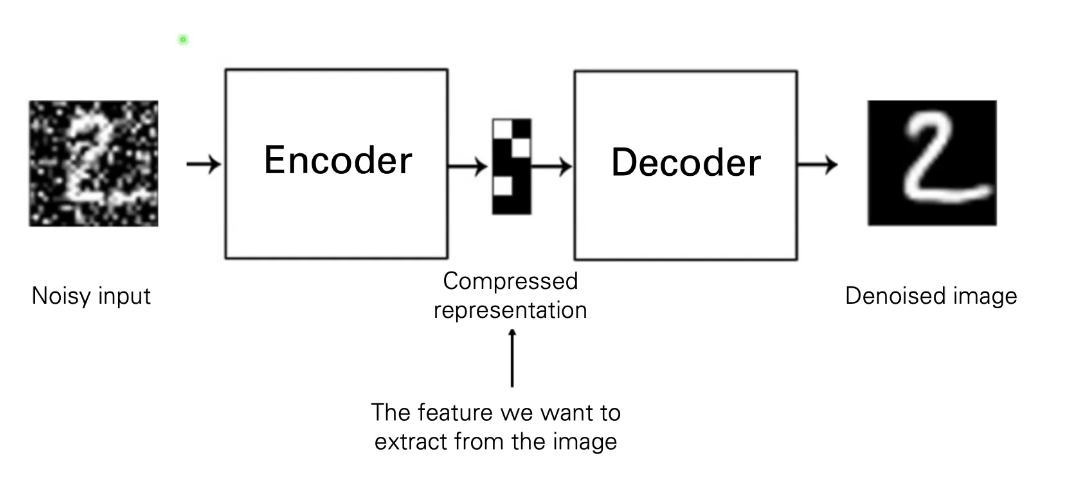
\includegraphics[width=0.8\linewidth]{figures/denoising_autoencoder.png}
   \caption{ Denoising Autoencoder}
   \end{figure}
 
Noises include stochasticity.
 
\par
What is happening is we are deforming the existing data sample in the existing data space.
The network should then separate noise from the actual image.
 
\textbf{Loss function} is weighted for this work in order to penalize
reconstructions of noisy pixels.
 
%
\begin{equation}
   L_{2, \alpha}
   (\mathbf{x}, \mathbf{z})
   =\alpha
   \left(\sum_{j \in \mathcal{I}(\tilde{\mathbf{x}})}\left(\mathbf{x}_{j}-\mathbf{z}_{j}\right)^{2}\right)
   +\beta\left(\sum_{j \notin \mathcal{I}(\tilde{\mathbf{x}})}\left(\mathbf{x}_{j}-\mathbf{z}_{j}\right)^{2}\right)
   \label{eq:denoising_autoencoder_loss_function}   
\end{equation}
%
 
 
Before 2010 the main dominant approach for training of neural networks
was to have a layered pretrained steps where you incrementally increase
the complexity of  the network and this work is one such example. Again
historically representations of neurons were included in the papers because
people were trying to find commonalities between neural representations
and mammal visual system.
 
\begin{figure}[H]
   \centering
   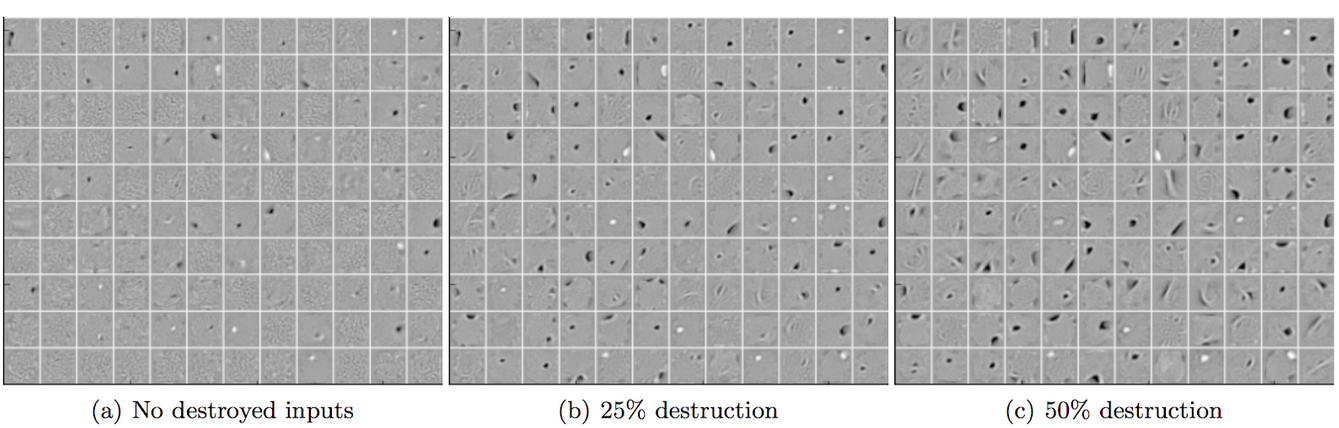
\includegraphics[width=0.8\linewidth]{figures/denoising_autoencoder_neuron_visualizition.png}
   \caption{ Neuron Visualization of Denoising Autoencoder under different destruction of the data}
   \end{figure}
 
Interestingly, when corruption level increases the network learns more from
the data.
 
 
\subsubsection{Predict Missing Pieces}
Task is to strip of some part of the image and then try to inpaint
stripped part with the neural networks.
Prominent and pioneer paper for this task is
"Context Encoders: Feature Learning by Inpainting" \cite{pathak2016context}
 
\begin{figure}[H]
   \centering
   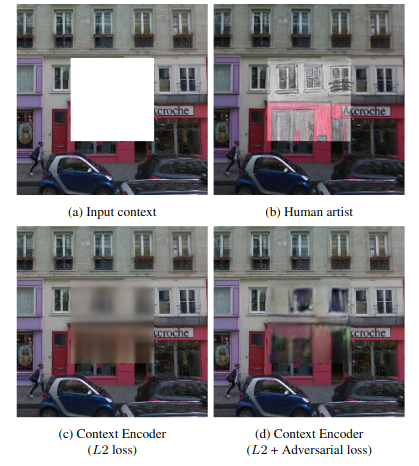
\includegraphics[width=0.8\linewidth]{figures/inpainting.png}
   \caption{ Qualitative illustration of the task.
   Given an im-age with a missing region (a),
   a human artist has no trouble inpainting  it  (b).
   Automatic  inpainting 
   using  our context encoder trained
   with L2 reconstruction loss
   is shown in (c),
   and using both L2 and adversarial losses in (d)}
   \end{figure}
 
   Context Encoder can be seen in figure 4.
   The context image is passed through
   the encoder to obtain features which are
   connected to the decoder using
   channel-wise fully-connected layer.
   The decoder then produces the missing regions in the image.
 
\begin{figure}[H]
       \centering
       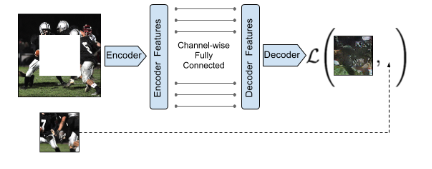
\includegraphics[width=0.8\linewidth]{figures/inpaintin_model.png}
       \caption{ Inpainting Model Overview}
       \end{figure}
 
 
Instead of just cutting the middle part of the image,
random blocks and shapes can be sampled for reconstruction.
 
Another contribution of the authors is also to use of adversarial loss
along with the reconstruction loss for this task.
 
\begin{figure}[H]
   \centering
   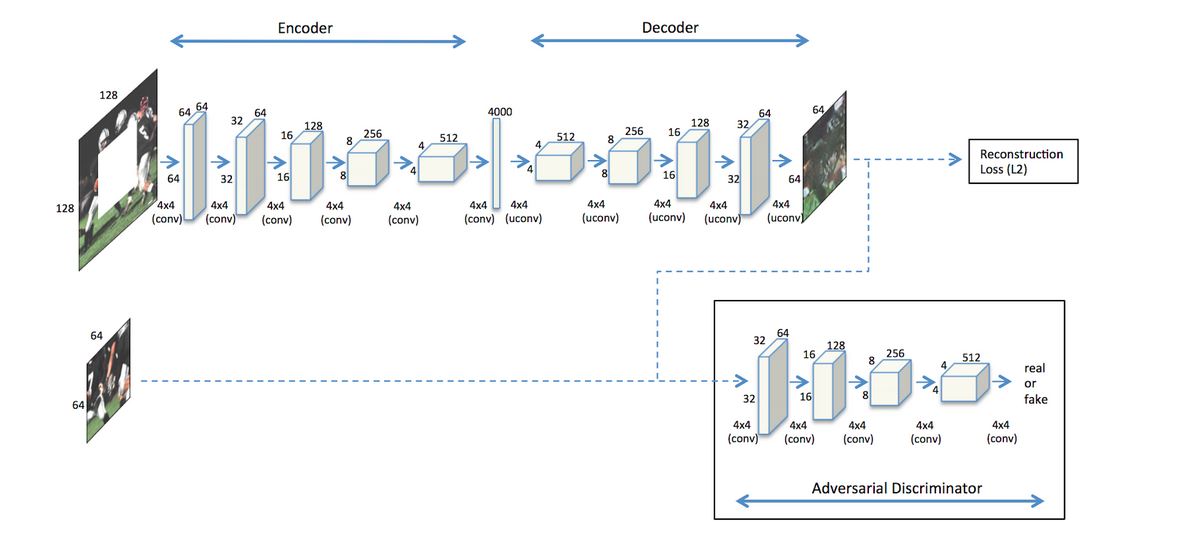
\includegraphics[width=0.8\linewidth]{figures/inpainting_detailed_overview_model.png}
   \caption{ Inpainting Detailed Model Overview: Context Encoder}
   \end{figure}   
 
As we have stated earlier though the main purpose for this approach is not to
be able to reconstruct or regenerate the pretext task but model to evolve
in a way that it can be useful for other downstream tasks.
Context encoders although a preliminary work it is actually reports
promising results for that time. Although is pretty much below to the
scores of ImageNet Pretrained models.
 
 
\subsubsection{Cross-Channel Autoencoder}
 
In Cross-Channel Autoencoder's \cite{DBLP:journals/corr/ZhangIE16a}
it is assumed that only single view of the input is accessed
and the purpose of this network is to reconstruct the other views.
 
\begin{figure}[H]
   \centering
   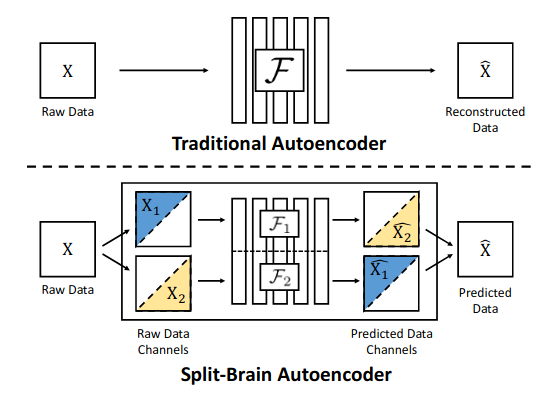
\includegraphics[width=0.8\linewidth]{figures/cross-channel-ae.png}
   \caption{Traditional  vs  Split-Brain  Autoencoder  architectures.
   (top)Autoencoders learn feature representation F
   by learning to reconstruct input dataX.
   (bottom)The proposed split-brain autoencoder
   is composed of two disjoint sub-networks
   F1, F2, each trained to predict one
   data subset from another, changing  the  problem 
   from reconstruction to prediction.
   The split-brain representation F
   is formed by concatenating the two sub-networks,
   and achieves strong transfer
   learning performance.
   The model is publicly available
   on https://richzhang.github.io/splitbrainauto.}
   \label{fig:split-brain}
   \end{figure}
 
\begin{figure}[H]
       \centering
       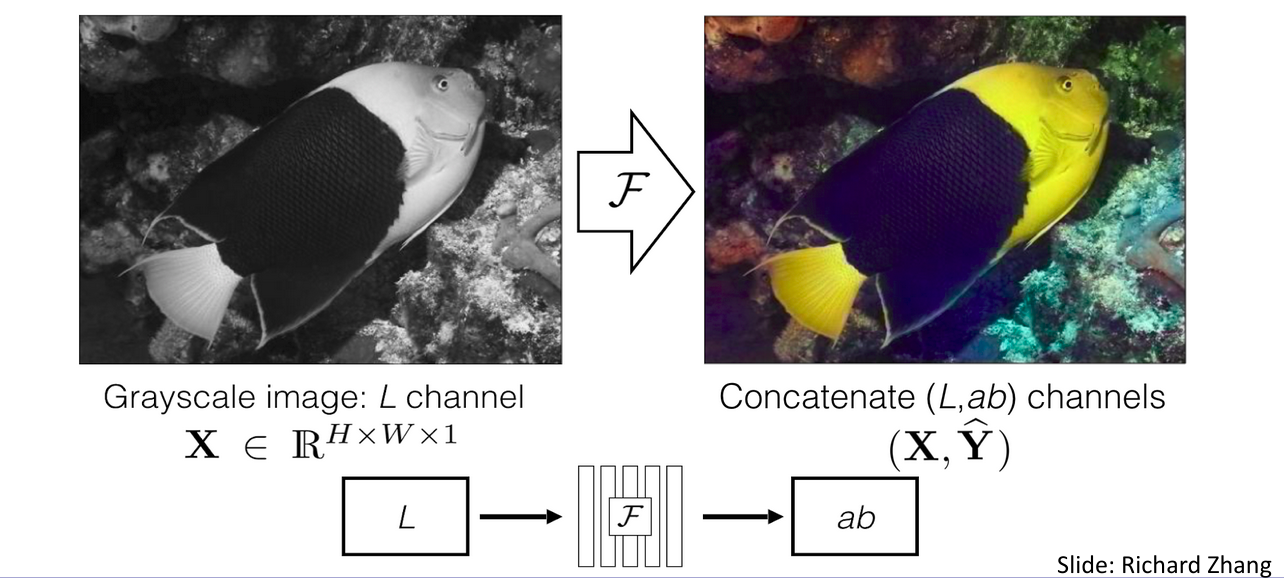
\includegraphics[width=0.8\linewidth]{figures/cross-channel-example.png}
       \caption{Image Colorization Example}
       \label{fig:cross-channel-example}
       \end{figure}
 
In \ref{fig:cross-channel-example} image colorization task can be seen.
In the figure the images are assumed to be in Lab color space.
So given L channel ab channels are predicted and in the end all
are concatenated.
 
For the objective again L2 loss is  used and also additionally pixel values
are treated as classes so they approached the problem as a pixel-wise
classification problem.
 
In \ref{fig:split-brain} you have basically two networks and each is given
the other channel as input and tries to predict the other.
So it can be said that those are complementing networks.
And in the end their output is combined to reconstruct the original input image.
 
\subsection{Proxy Tasks In Computer Vision}
 
\subsubsection{Relative Patch Prediction}
Task is to predict the relative position of the second patch
with respect to the first.
\begin{figure}[H]
   \centering
   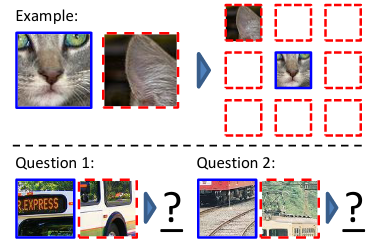
\includegraphics[width=0.8\linewidth]{figures/proxy-task-context-prediction.png}
   \caption{Learning Patch Representation}
   \label{fig:learning_patch_representation}
   \end{figure}
 
 
   Architecture in the \ref{fig:patch_model} is for pair classification.
   Dotted lines indicate shared weights and
   ‘LRN’ is a local response normalization layer.
   All conv and fc layers are followed by ReLU nonlinearities,
   except fc9 which feeds into a softmax classifier.
   So it is a pretty standard "Siamese" sort of architecture.
 
\begin{figure}[H]
       \centering
       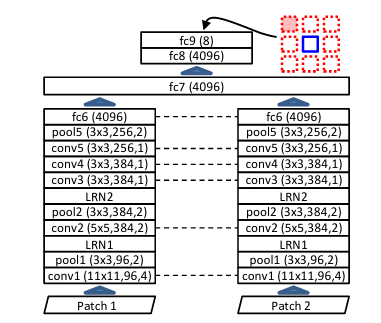
\includegraphics[width=0.8\linewidth]{figures/proxy_task_context_patch_network.png}
       \caption{"Unsupervised Visual Representation Learning by Context Prediction" \cite{doersch2016unsupervised} Neural Network Architecture}
       \label{fig:patch_model}
       \end{figure}
 
 
\subsubsection{Solving Jigsaw Puzzles}
The tasks that we are dealing today actually consecutive works meaning
that they share much incrementally improves the previous works.
 
Solving jigsaw puzzles follows this fashion.
In that instead of just correctly guessing position of patches,
this model is given with all the patches but all patches are shuffled.
What this does is to correctly fix the position of the patches in order to
form original image. This models network architecture is very similar to
patch model and task is again classification.
 
\begin{figure}[H]
   \centering
   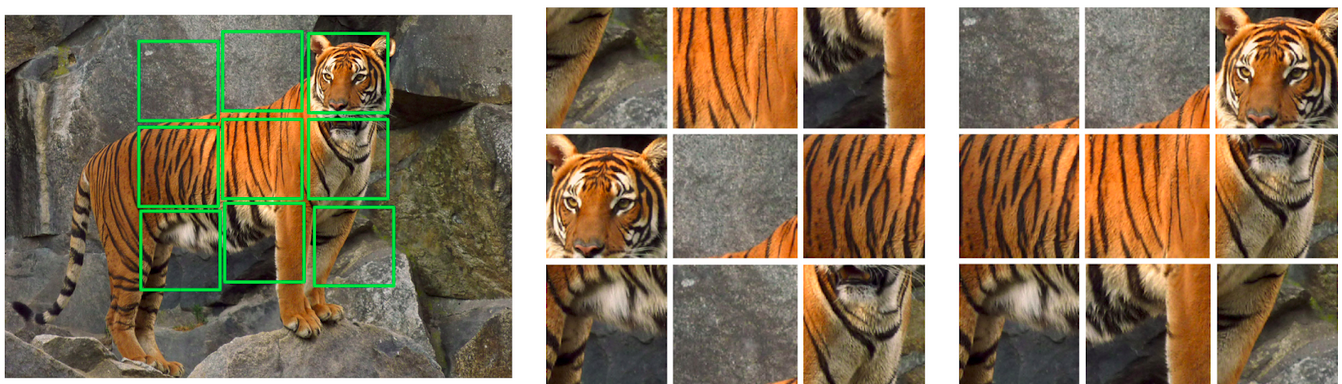
\includegraphics[width=0.8\linewidth]{figures/jigsaw.png}
   \caption{Solving Jigsaw Puzzle Task Representation}
   \label{fig:jigsaw_task}
   \end{figure}
 
 
\subsubsection{Rotation}
 
Rotation task is to predict whether the given image is rotated or not and
if it is rotated, the rotation angle should be determined as well.
Again this problem is attacked in a way that is turned into a classification
problem and the output is one of the four classes and multiples of 90 degrees.
In order to correctly predict the rotations the model should have an understanding
of the image and its correct rotation. So hopefully model learns what the object is
maybe. And because of that although the approach is easy, its results are better
than other self supervised models we learned so far.
\begin{figure}[H]
   \centering
   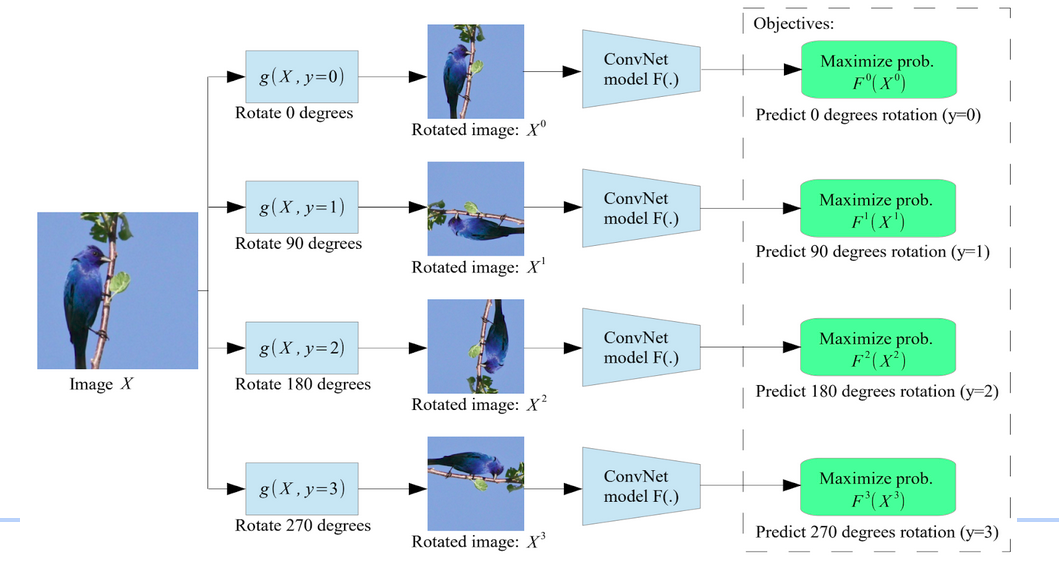
\includegraphics[width=0.8\linewidth]{figures/rotation_model.png}
   \caption{Rotation Task and The Model Architecture \cite{DBLP:journals/corr/abs-1803-07728}}
   \label{fig:rotation_model}
   \end{figure}
 
 
\subsubsection{Temporal Coherence of Color}
Task given a color video colorize all frames of a grayscale version
using a reference frame for guidance.
Main motivation for this task is to get an understanding of
the environment and the objects in different frames and
try to associate them with each other in different frames.
So it can be said that tracking emerges from colorization.
 
\begin{figure}[H]
   \centering
   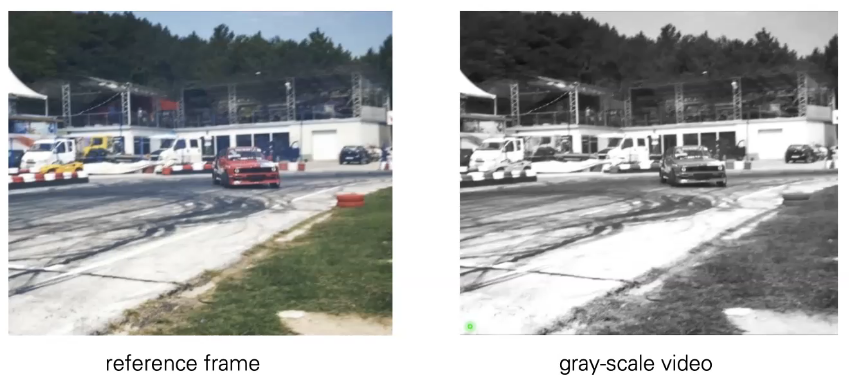
\includegraphics[width=0.8\linewidth]{figures/temporal_coherence_color.png}
   \caption{Temporal Coherence of Color Task Visualization}
   \label{fig:temporal_coherence_color}
   \end{figure}
 
\subsection{Contrastive Learning}
So far we needed to design a proxy task to have better representation
learning schema.
Now we would be mostly concentrating on a single objective trying to
distinguish whether a pair of data samples are similar to each other or
dissimilar to each other.
 
As a motivating example we will now focus on "Word2Vec" \cite{mikolov2013efficient} which led to
huge improvements in deep learning specifically in natural language processing.
 
\subsubsection{Word2Vec}
Forming word embeddings is a problem.
One hot vector encoding approach can be speculated.
But that is very sparse and requires a dimension for
each new word and has no semantic relation because of
orthogonality.
So this is a naive way of embedding words.
 
Because of the inadequacy of one-hot word representations
distributional representations of words had been investigated.
It means each word gains meaning in response to its neighbors.
So the meaning arises from context. This is one of the most successful
ideas in NLP.
 
\textbf{The meaning of a wampimuk(guess what this word is :) ) is (can be approximated by, derived
from ) the set of contexts in which it occurs in texts.}
 
\par
In W2V model n-gram language modeling idea is used.
 
\textbf{Unigram}
\begin{equation}
   P\left(w_{1}, w_{2}, \cdots, w_{n}\right)
   =\prod_{i=1}^{n} P\left(w_{i}\right)
   \end{equation}
 
\textbf{Bigram}
\begin{equation}
       P\left(w_{1}, w_{2}, \cdots, w_{n}\right)=
       \prod_{i=2}^{n} P\left(w_{i} \mid w_{i-1}\right)
\end{equation}
 
W2V paper involves two implementations.
The first is a continuous bag of words.
The other is skipgram.
Importance negative sampling is used for propagation of supervision.
 
 
\begin{figure}[H]
   \centering
   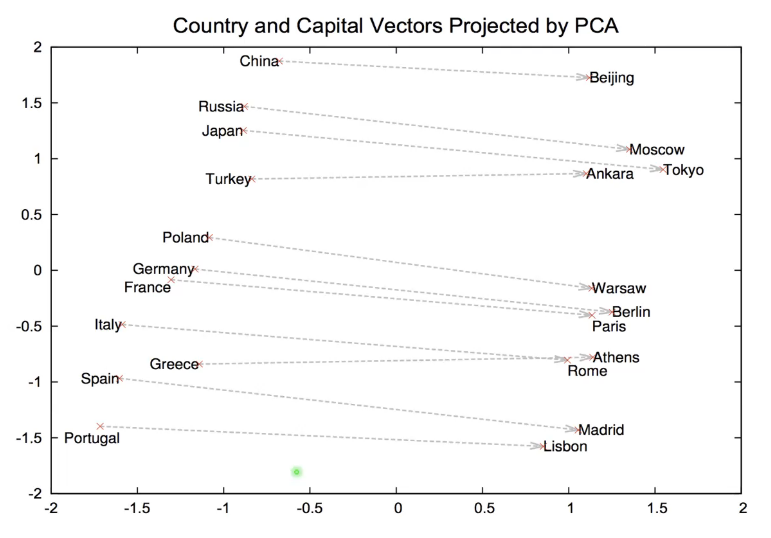
\includegraphics[width=0.8\linewidth]{figures/w2v_semantic.png}
   \caption{Semantic Embeddings of W2C}
   \label{fig:w2c_semantic}
   \end{figure}
 
Learned embeddings from Word2Vec model are quite semantic.
It captures semantic relations between words.
In \ref{fig:w2c_semantic} it can be seen that vectoric relations are present
in the differences of word embeddings.
 
\par
Another important paper in this line of works is "Deep InfoMax" \cite{hjelm2019learning}.
Input image is encoded into a grid structure by MxM feature map.
Each feature is a vector.
Vectors might be different for different classes of objects.
And the idea is to maximize the encoder input and output.
If you consider from the features corresponding features should be
similar to the global feature of this input image.
As a result we want to maximize shared information between global features and
local features.
Hence, local representations would become representatives of global features.
So images would be distinguished by their local features.
Classification accuracy results for this paper are superior for its time.
 
\begin{figure}[H]
   \centering
   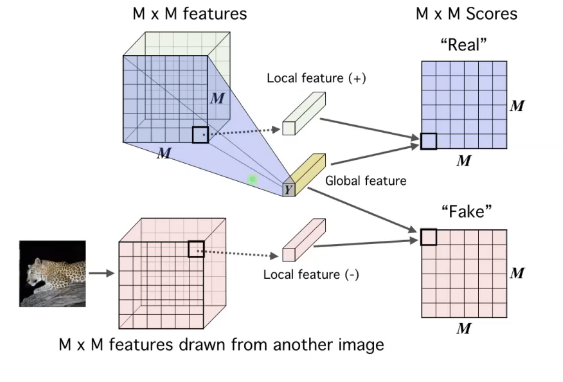
\includegraphics[width=0.8\linewidth]{figures/deepinfo_max.png}
   \caption{DeepInfo Max Model}
   \label{fig:deepinfomax_model}
   \end{figure}
 
 
\textbf{Contrastive Loss,} is the indication of similarity and dissimilarity between
vectors and in "DeepInfoMax" this is what we are trying to reduce between local
and global features.
 
\subsubsection{Contrastive Predictive Coding}
\cite{DBLP:journals/corr/abs-1807-03748}, the main idea of this paper is
supposingly instead of having generative loss we have encoding and decoding.
Very much like to DeepInfoMax approach, we may try to maximize mutual information
between sequences of data. So again in the CPC approach we need to have negative samples as well.
 
\begin{figure}[H]
   \centering
   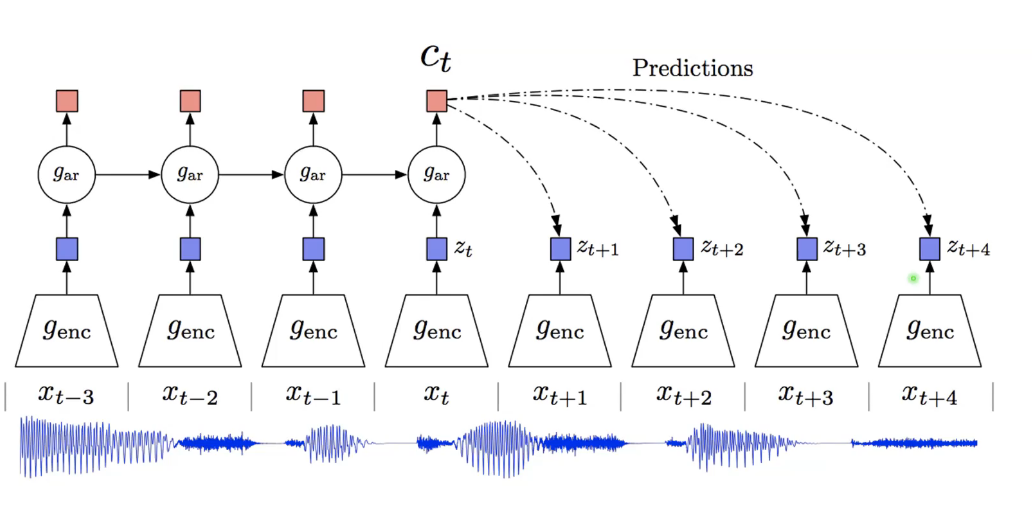
\includegraphics[width=0.8\linewidth]{figures/cpc.png}
   \caption{CPC Approach}
   \label{fig:cpc}
\end{figure}
 
With this manner you can learn much more semantic and slowly varying features.
Really useful features can be extracted as a result.
 
Main idea in contrastive predictive coding is that we assume a particular
context is observed regarding our data.
Instead of just generating what comes next as in a classical Autoregressive
sense, here we we would like to predict not the original input but
latent codes that are obtained by some encoder. That constitutes the prediction stage.
What makes it contrastive is the usage of contrastive loss.
 
\begin{figure}[H]
   \centering
   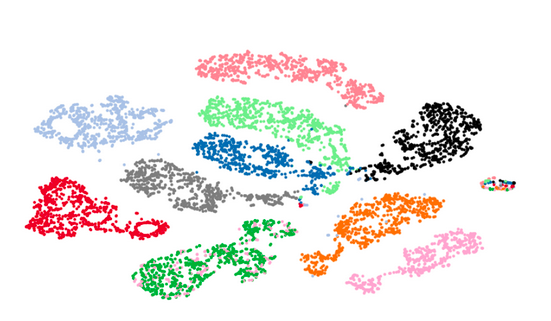
\includegraphics[width=0.8\linewidth]{figures/tsne_cpc_speech.png}
   \caption{t-SNE visualization of audio (speech) representations for
   a subset of 10 speakers (out of 251). Every color represents a different speaker}
   \label{fig:cpc_speech}
\end{figure}
 
\textbf{CPC - Speech: } In \ref{fig:cpc_speech}, it can be seen that
the embeddings of input for the same users(speakers) clustered together.
Thus we can infer that the model learned the characteristics of speakers
from unlabeled data.
 
\textbf{CPC - ImageNet: } CPC framework is a generic one and can be used with
other modalities. As an example in visual domain we can apply cpc by
creating overlapping image patches and encoding them. After creating the
encodings the idea is the same. Can we predict the other representations?
Quite basic autoregressive task in the latent space.
What expected is from our encoders then is to be able to encode what the
object of patch is. So that it can predict the following image patches.
 
\begin{figure}[H]
   \centering
   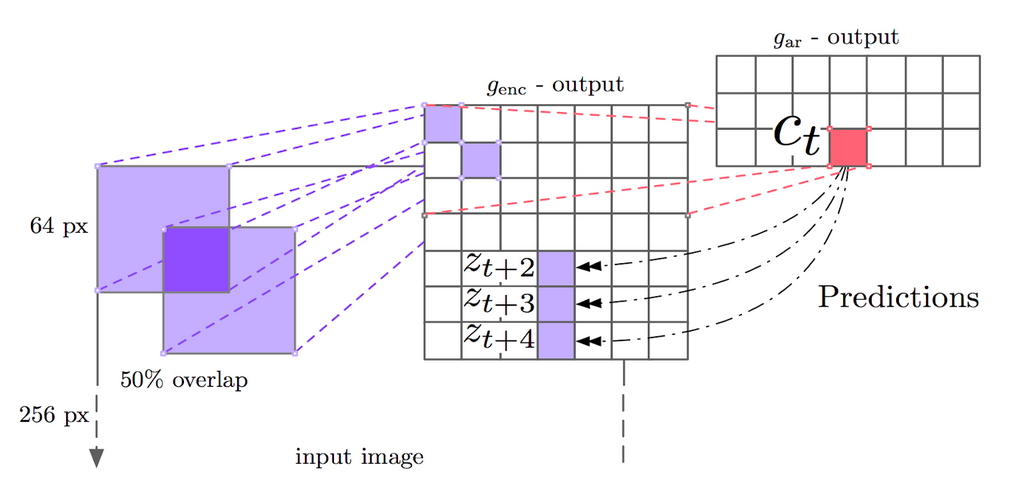
\includegraphics[width=0.8\linewidth]{figures/cpc-imagenet.png}
   \caption{Visualization of CPC for Images}
   \label{fig:cpc_imagenet}
\end{figure}
 
CPCV2 \cite{henaff2020data}: This work is very important turning
point for self-supervised learning and CPC. The idea and the framework
is the same. Only some changes are introduced for implementation.
This model predicts the next couple of rows. However, pixel cnn sort of approach would be
better and more efficient.
This model computes similarity between contextual features and
other latent codes. We want to compute it using some feature transformation.
And we still need negative samples either from same image or from different
images from the dataset.
Loss is very similar to Word2Vec approach and InfoNCE(Noise Contrastive Estimation)
loss is used.
 
 
Main advantage comes from the followings:
 
\begin{itemize}
   \item Very large dataset is used (Unlabeled ImageNet)
   \item Long training time (500 epochs and 1 week)
   \item Larger patch size
   \item Effective number of negative samples
   \item \textbf{Augmenting every patch with a lot
   of spatial and color augmentations}
\end{itemize}
 
They can even exceed the performance of supervised baseline
which is the first time for this self supervised approach.
 
We can again understand the importance of self-supervised learning
by looking at the outcomes of this research. Because it allows
more efficient way to train our classifiers as compared to the
supervised approaches after the pretraining stage.
 
\begin{figure}[H]
   \centering
   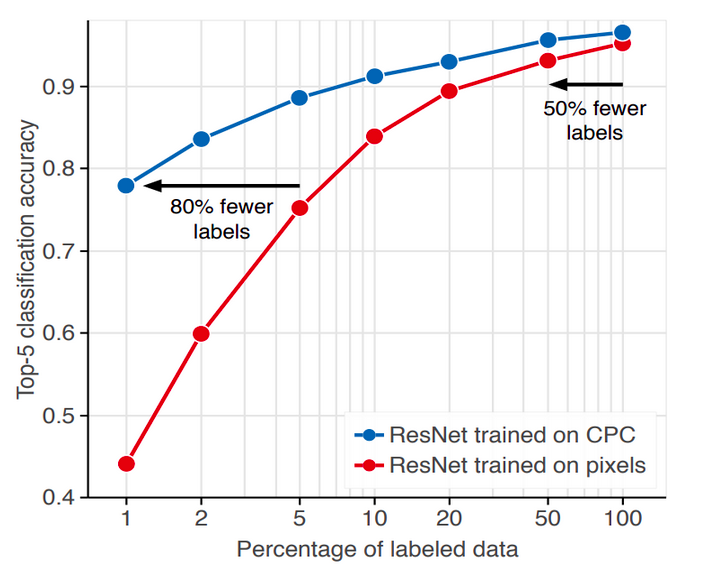
\includegraphics[width=0.8\linewidth]{figures/cpcv2_eff.png}
   \caption{Data Efficiency of CPC V2}
   \label{fig:cpc_v2_eff}
\end{figure}
 
 
 
\subsection{Momentum Contrast (MoCo) \cite{he2020momentum}}
 
 
\begin{figure}[H]
   \centering
   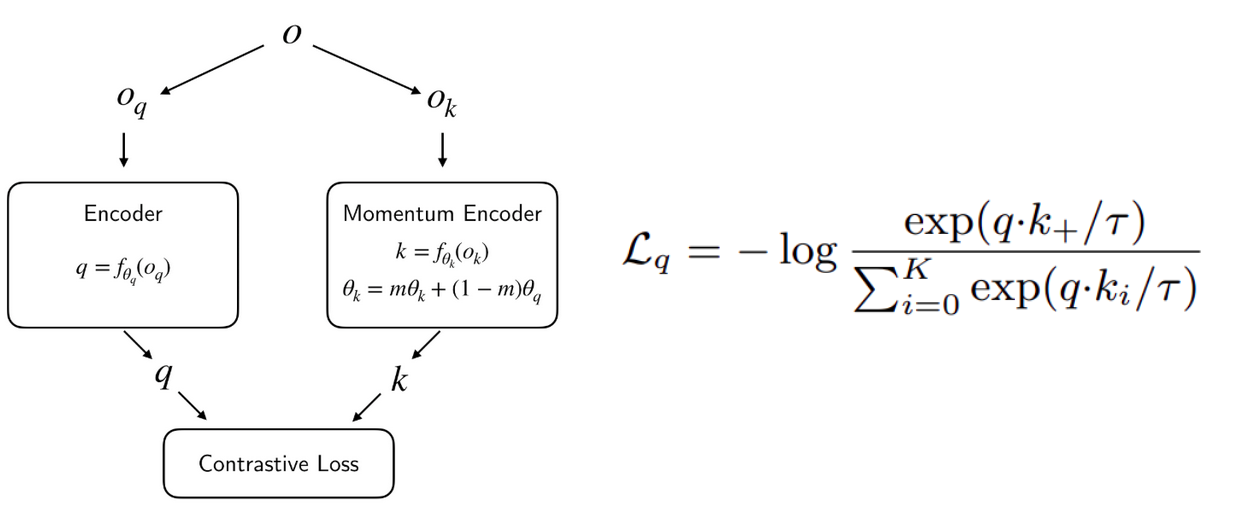
\includegraphics[width=0.8\linewidth]{figures/moco.png}
   \caption{MoCo Overview and Loss Function}
   \label{fig:moco}
\end{figure}
 
MoCo, checks whether two data instances are similar or not.
Does it so by using contrastive loss.
As a result, the model outputs similarity representations.
 
Main idea for MoCo is not using the same encoder for both parts.
Thus, it introduces momentum encoder for the key part.
 
Critical thing for MoCo to be effective is to update
weights of momentum encoder not in every step but basically
update it at some certain intervals.
 
When update takes place, it uses momentum idea and makes use of weights
of query encoder as well. This adds stability to the training.
 
When model capacity is maxed it even surpasses CPCv2 in terms of accuracy.
 
\subsection{Simple Framework for Contrasive
Learning of  Visual Representations (SimCLR) \cite{chen2020simple}}
 
\begin{figure}[H]
   \centering
   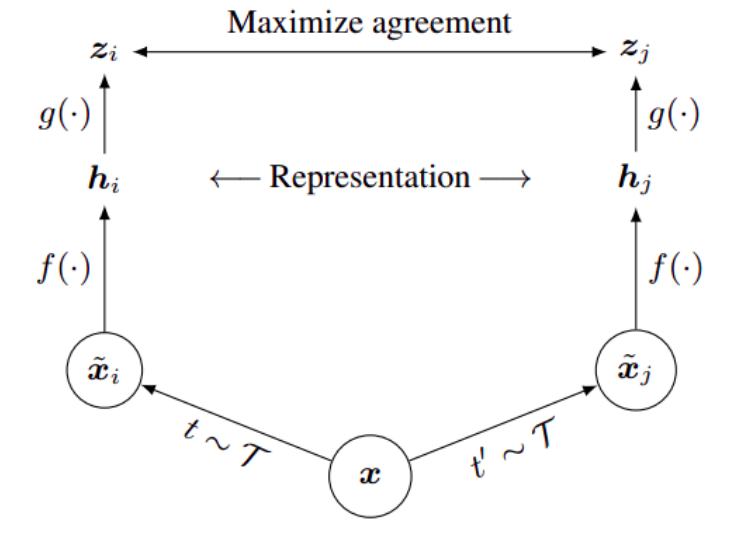
\includegraphics[width=0.8\linewidth]{figures/simclr.png}
   \caption{SimCLR Overview}
   \label{fig:simclr}
\end{figure}
 
Main idea of SimCLR is the use of projection head on top of
encoded features. Projection head is a simple MLP.
This model looks for agreement in transformed space.
Data augmentation strategies are used.
Distinguishes if transformed feature vectors are from the same
source or not.
In top-1 accuracy for ImageNet, accuracy is much better compared to
MoCo and CPCv2.
 
Inspired from this work MoCoV2 is presented.
The ideas added on top of MoCo are the followings:
 
\begin{itemize}
   \item MLP Projection head
   \item Augmentation with extra blur
   \item Cosine learning rate schedule
\end{itemize}
 
After those improvements MoCov2 surpasses SimCLR in terms of accuracy.
 
 
\subsection{Bootstrap Your Own Latent A New Approach
to Self-Supervised Learning (BYOL) \cite{grill2020bootstrap}}
 
\begin{figure}[H]
   \centering
   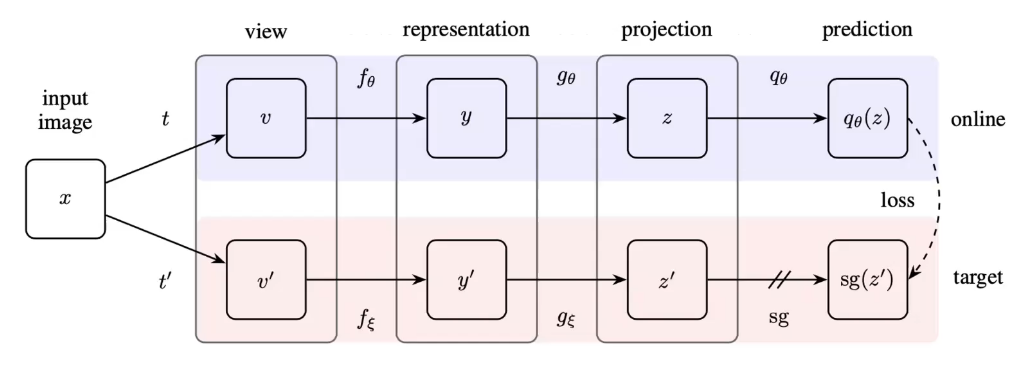
\includegraphics[width=0.8\linewidth]{figures/byol.png}
   \caption{BYOL Architecture and Overview}
   \label{fig:byol}
\end{figure}
 
BYOL borrows ideas from both MoCo and SimCLR.
The general flow is as follows:
\begin{itemize}
   \item perform some data augmentation
   \item generate two different views of the input Image
   \item Represent them using encoders
   \item Get projections of encodings from an MLP layer.
\end{itemize}
 
However, in contrast to other models BYOL does not use contrastive loss.
It instead tries to predict the latent of the other data (query latent).
Just as in MoCo query part of the model is not updated frequently and being updated
by using exponential moving average idea plus stop gradients.
 
Main distinction of the BYOL from other papers is that \textbf{it does not
use any negative samples at all!} and impressively performs a lot better
that all the previous models that we have seen so far. In fact it even outperforms
supervised peers in some datasets and tasks.
 
\begin{figure}[H]
   \centering
   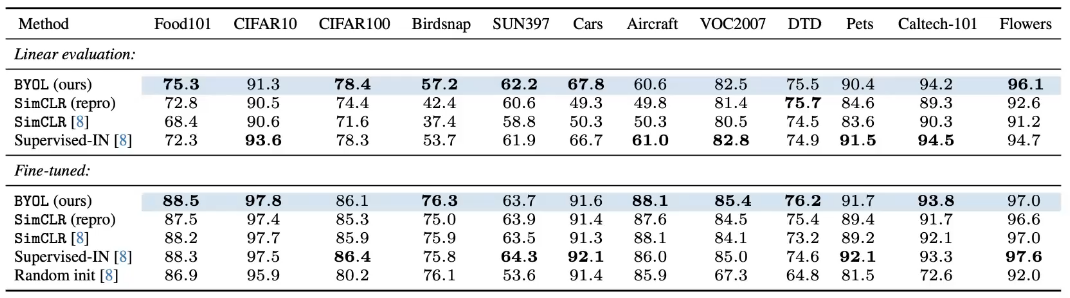
\includegraphics[width=0.8\linewidth]{figures/byol_results.png}
   \caption{BYOL, transfer learning results from ImageNet(IN)
   with the standard ResNet-50 architecture}
   \label{fig:byol_results}
\end{figure}
 
\bibliographystyle{plain}
\bibliography{bibliography_strings, bibliography_self_supervision}
 
\end{document}
 
 
 

